\begin{figure*}[t]
	\centering
	\begin{tabular}{cccc}
		\hspace{-0.5em}\subfloat[][$\sesync$]{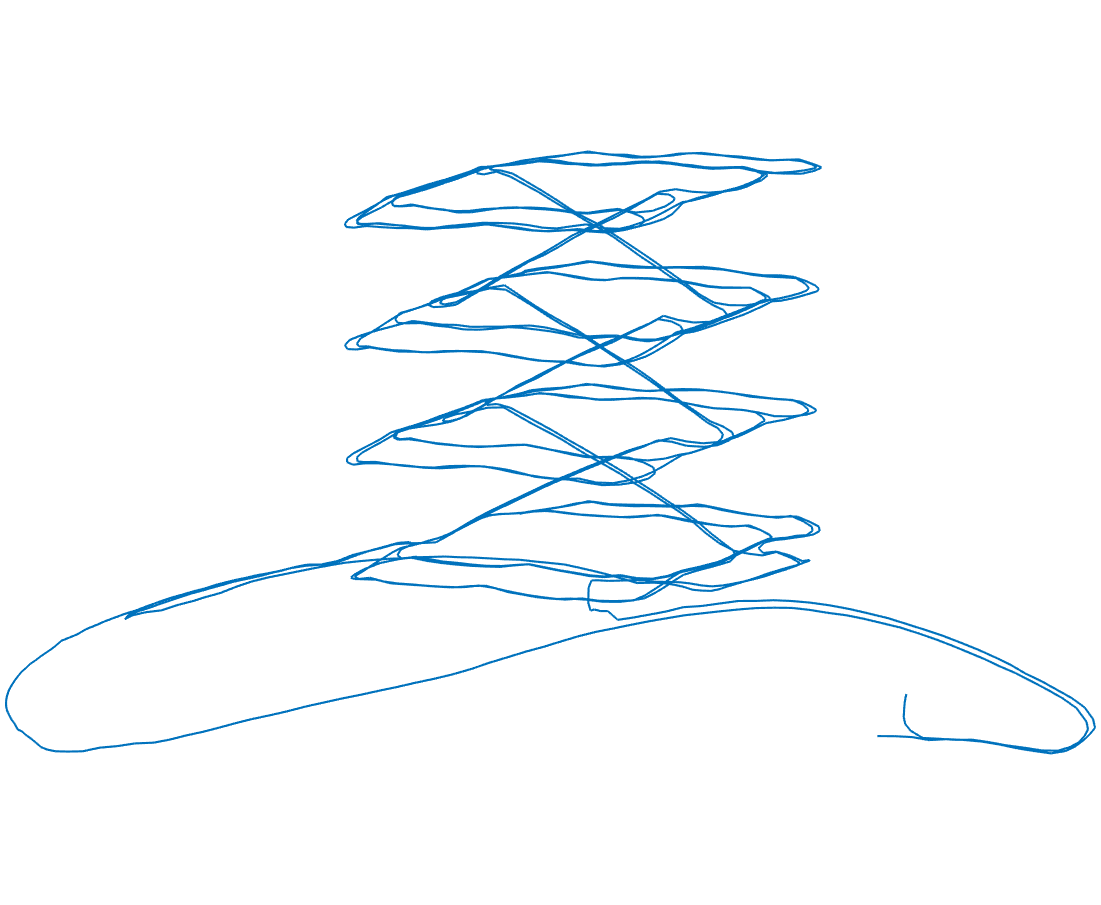
\includegraphics[trim =0mm 45mm 0mm 40mm,width=0.21\textwidth]{figures/outlier/garage_gt.png}} &
		\hspace{-0.6em}\subfloat[][The trivial loss kernel]{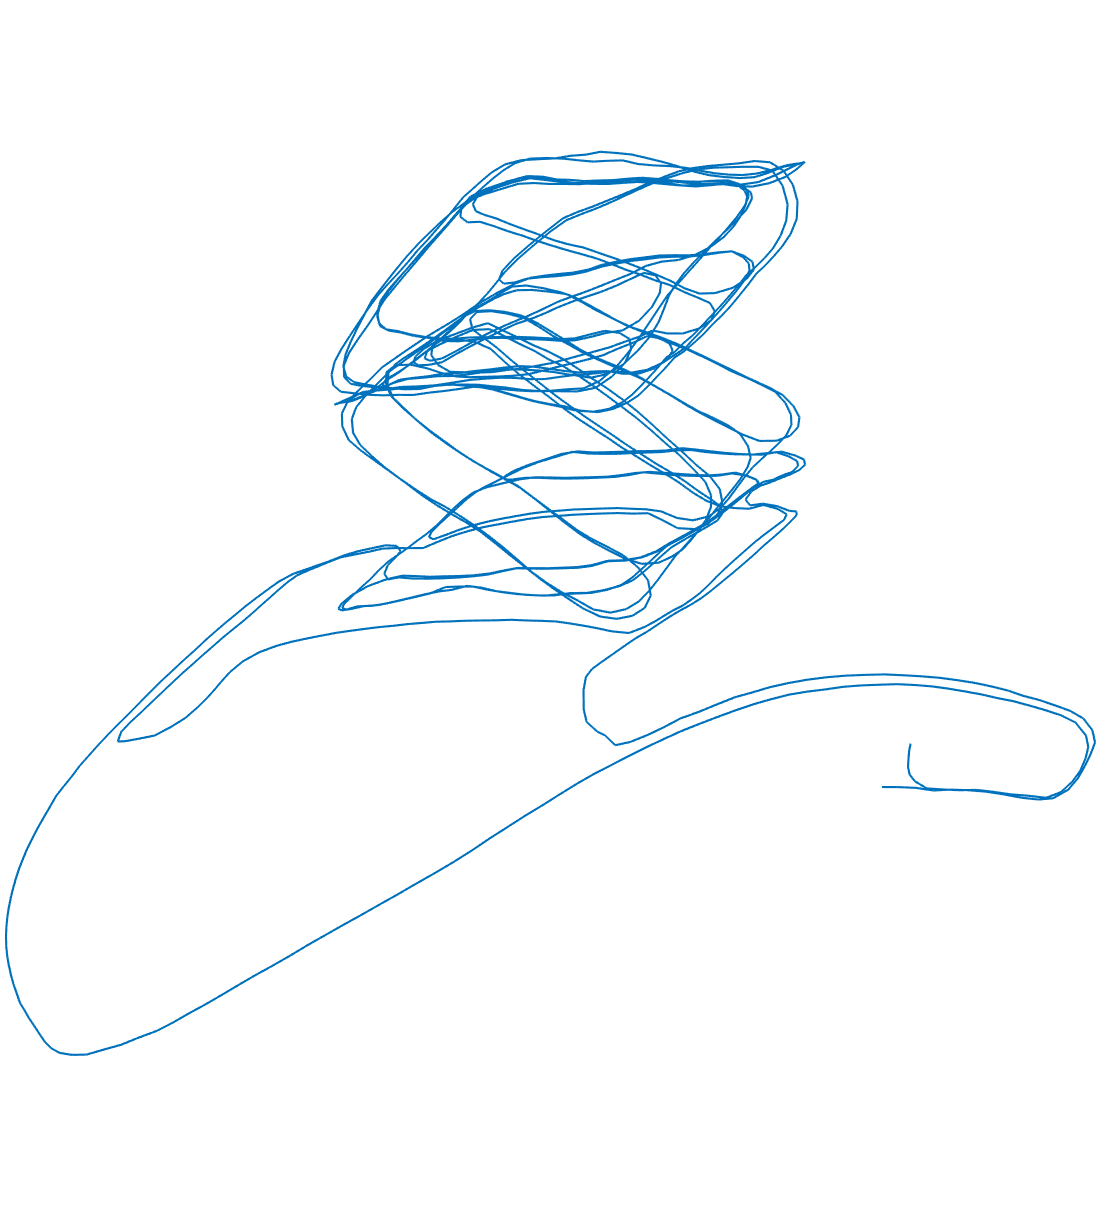
\includegraphics[trim =0mm 45mm 0mm 40mm,width=0.21\textwidth]{figures/outlier/garage_trivial.png}} &
		\hspace{-0.6em}\subfloat[][The Huber loss kernel]{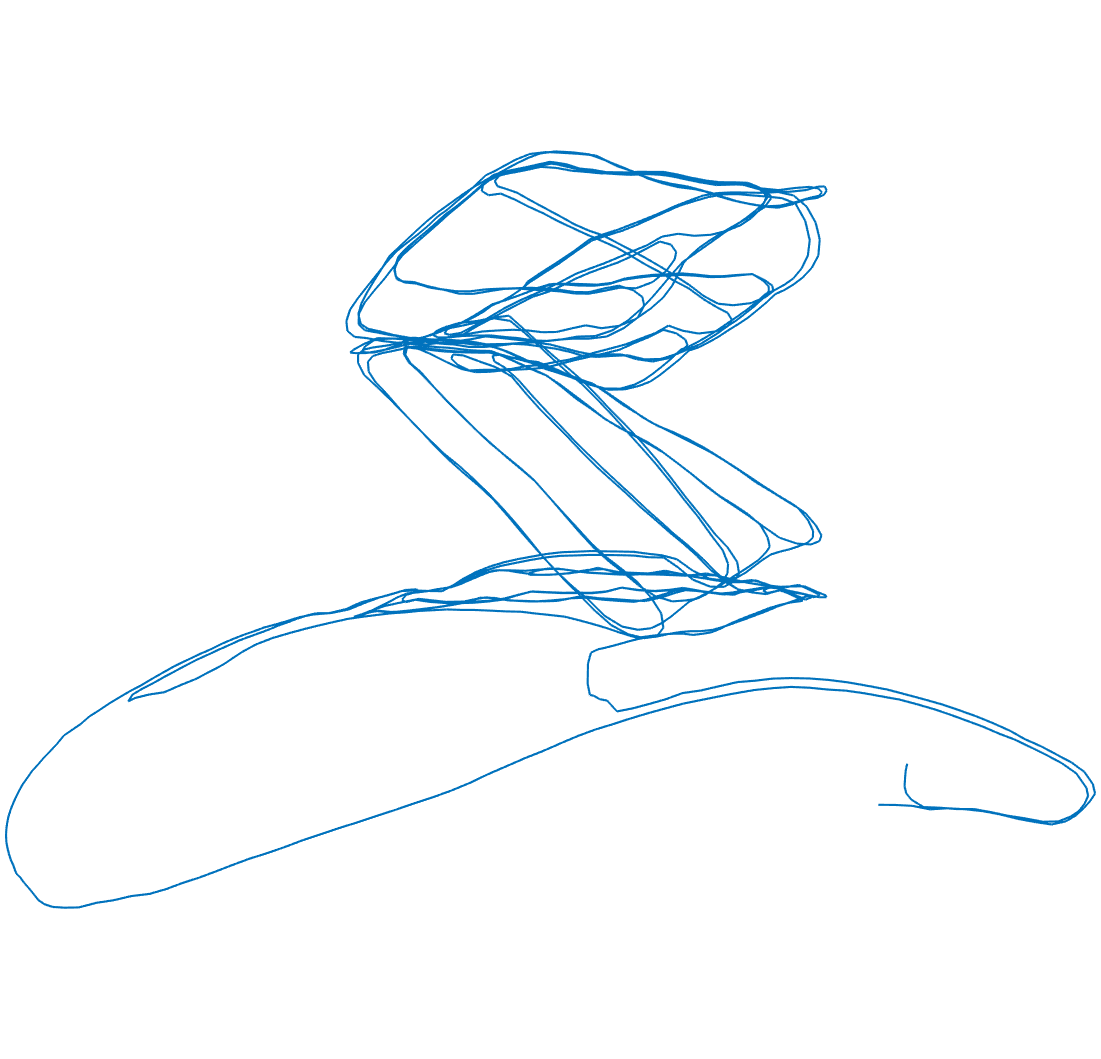
\includegraphics[trim =0mm 45mm 0mm 40mm,width=0.21\textwidth]{figures/outlier/garage_huber.png}}&
		\hspace{-0.6em}\subfloat[][The Welsch loss kernel]{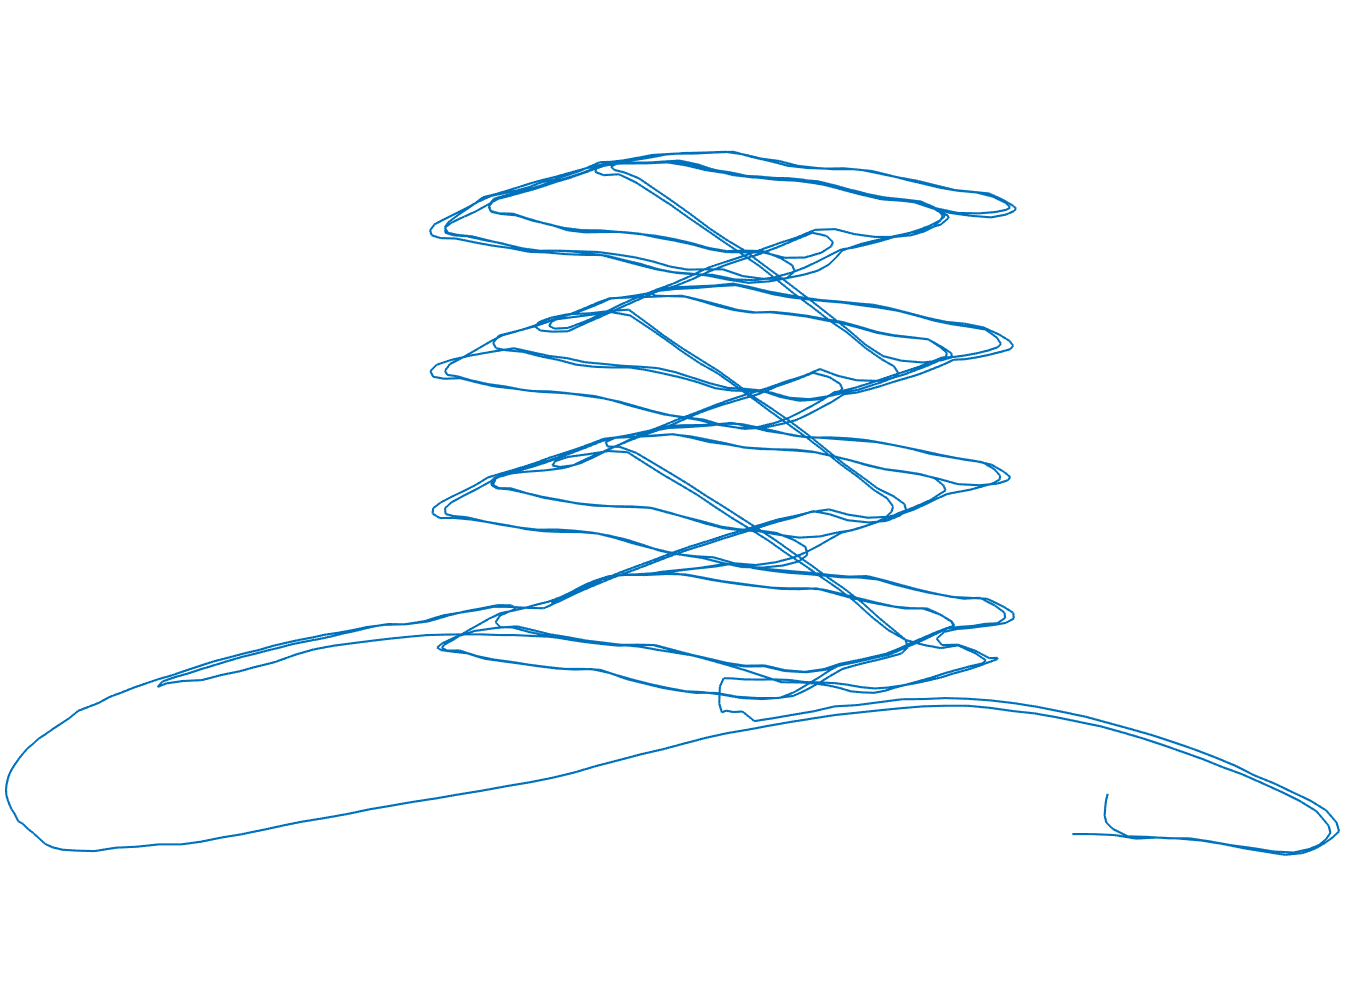
\includegraphics[trim =0mm 45mm 0mm 40mm,width=0.21\textwidth]{figures/outlier/garage_welsch.png}}
	\end{tabular}
	\caption{Qualitative comparisons of distributed PGO with the trivial, Huber and Welsch loss kernels for the {\sf garage} dataset with spurious inter-node loop closures. The outlier-free result of $\sesync$ \cite{rosen2016se} is shown in \cref{fig::outlier_garage}(a) for reference. The {\highlight outlier ratio} of inter-node loop closures is 0.6 and $\pcm$ \cite{mangelson2018pairwise} is used for initial outlier rejection. }\label{fig::outlier_garage}
	\vspace{-1.25em}
\end{figure*}